% pdflatex + distribution fonts only; no OS font dependency.
\usepackage[T1]{fontenc}
\usepackage{times}
\usepackage{amsmath,amssymb}
\usepackage{graphicx,booktabs,array}
\usepackage{tikz}
\usetikzlibrary{arrows.meta,calc,backgrounds}
\usepackage{cite}
\usepackage{balance}
\usepackage{capt-of}
\usepackage[hidelinks]{hyperref}
\hypersetup{pdftitle={Splatt3R-SLAM: From Image Pairs to Persistent Maps}}
\ifralreview
  \hypersetup{pdfauthor={}}
\else
  \hypersetup{pdfauthor={Zelong Li}}
\fi
\newcommand{\method}{Splatt3R-SLAM}
\newcommand{\best}[1]{\textbf{#1}}
\newcommand{\dB}{\,dB}
\newcommand{\up}{$\uparrow$}
\newcommand{\dn}{$\downarrow$}
\graphicspath{{ral/fig/}}
\IEEEaftertitletext{%
  \begin{minipage}{\textwidth}
    \centering
    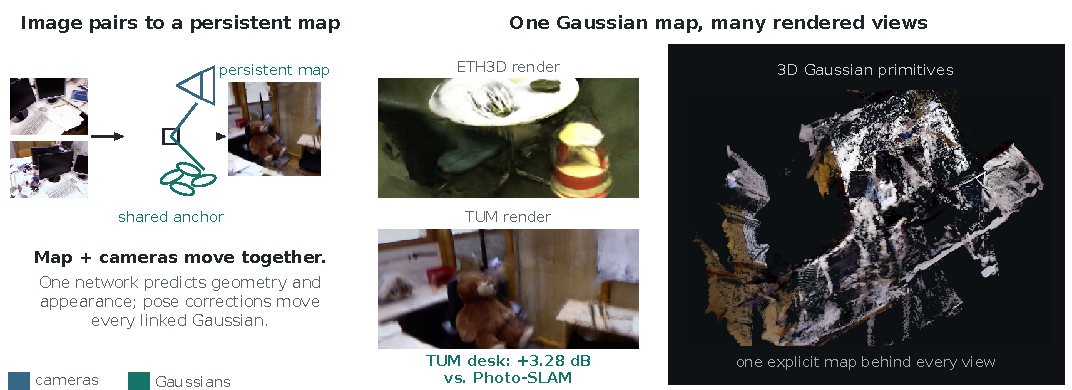
\includegraphics[width=\textwidth]{teaser.pdf}
    \captionof{figure}{\textbf{Pairwise predictions become a persistent map.}
    (a) A pose correction moves a local map and its observation cameras
    together; grey shows their previous positions.
    (b) Common-camera renderings with identical crops.
    (c) Mean PSNR on all eight Replica scenes: 23.02\,dB for Splatt3R-SLAM
    versus 19.48\,dB for Photo-SLAM, with eight scene wins.
    Results use 300\,s polish, non-keyframe cameras and full exported SH.}
    \label{fig:teaser}
  \end{minipage}\vspace{10pt}%
}
